\section{Zielsetzung}
In diesem Versuch soll die Dampfdruckkurve von Wasser bestimmt werden.
Dafür wird der Übergang zwischen den Phasen flüssig und gasförmig untersucht.

\section{Theoretische Grundlagen}
Stoffe haben die Möglichkeit unter bestimmten Bedingungen drei verschiedene Phasen anzunehmen.
Die Phasen sind hier die Aggregatzustände fest, flüssig und gasförmig.
In einem Zustandsdiagramm wie in Abbildung (\ref{fig:zustand}) kann die Phasenverteilung graphisch dargestellt werden.

\begin{figure}
  \centering
  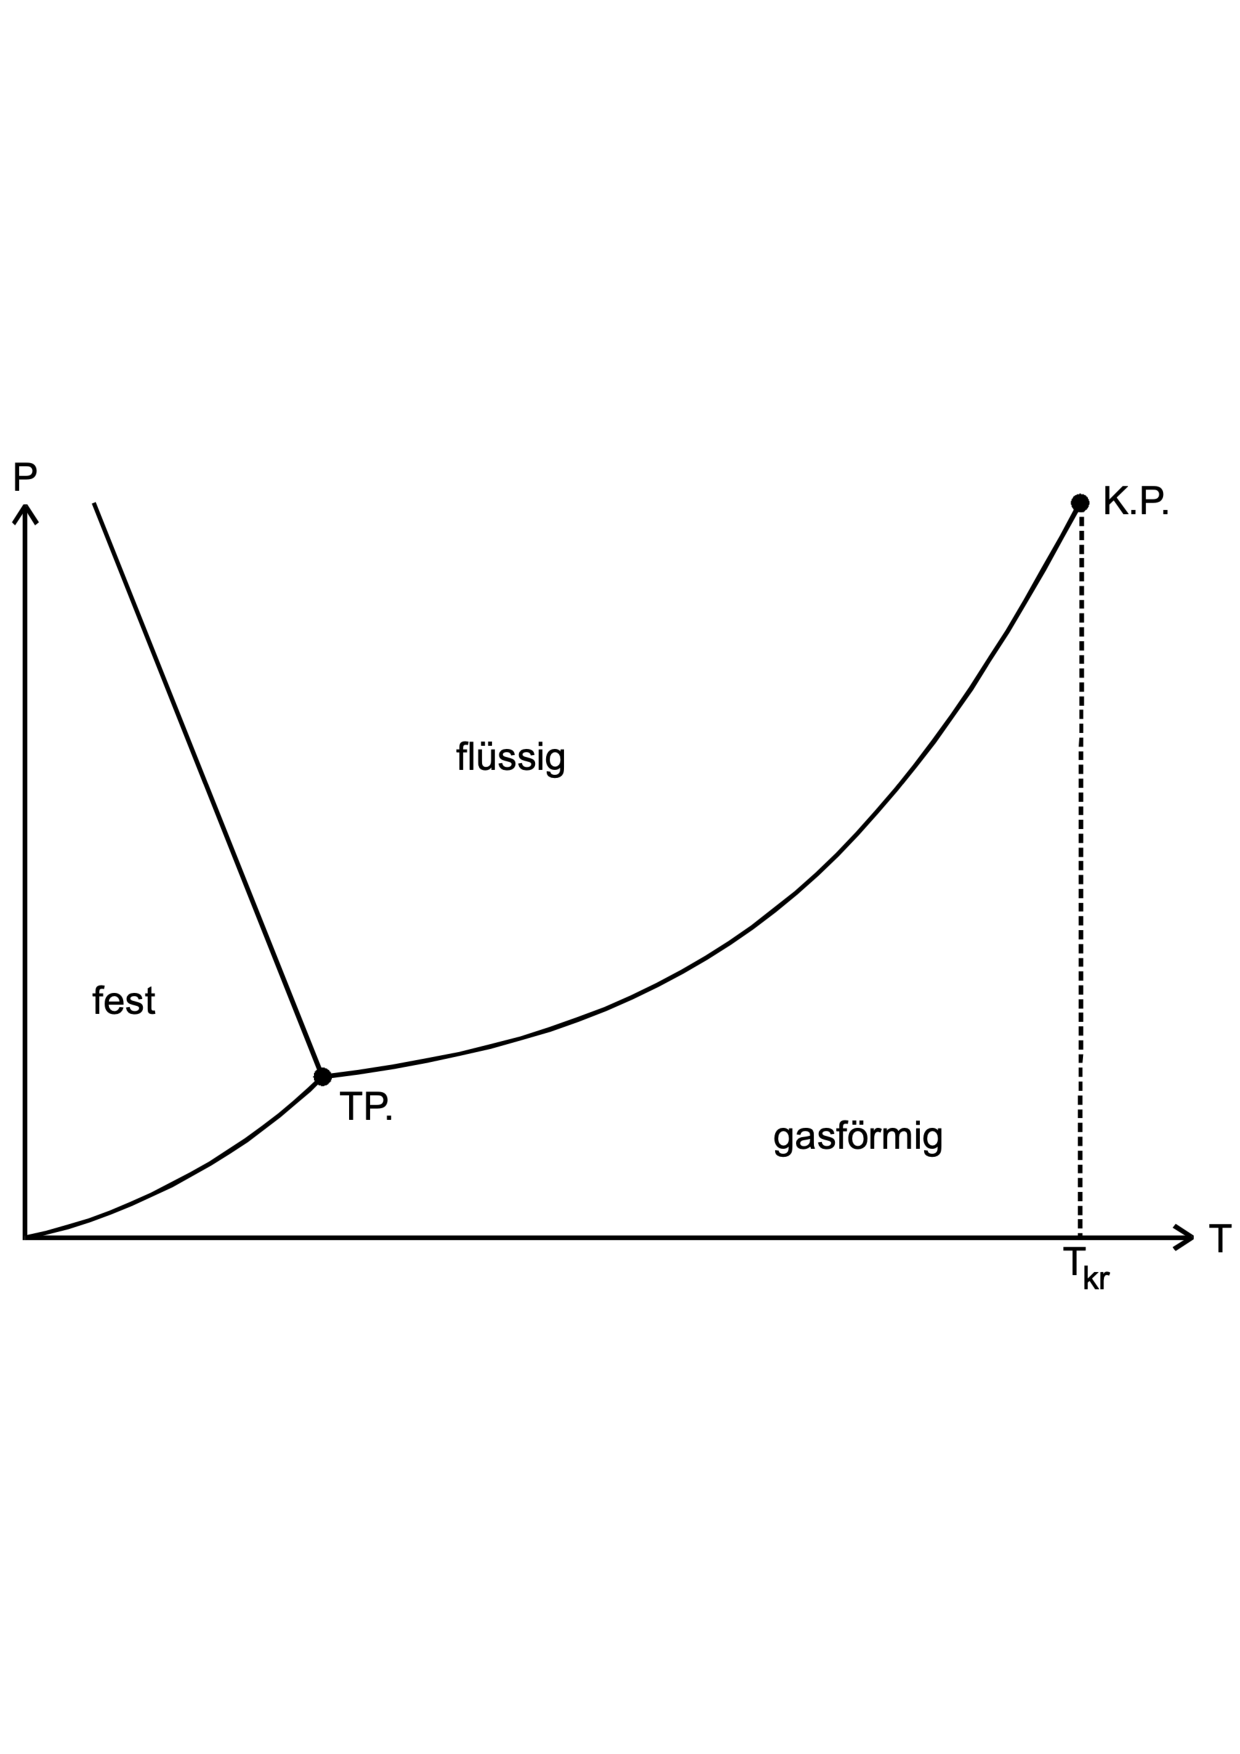
\includegraphics[width=8.5cm]{zustand.pdf}
  \caption{Qualitatives Zustandsdiagramm von Wasser \cite{V203}.}
  \label{fig:zustand}
\end{figure}

\noindent
Im p-T-Diagramm kennzeichnen die Linien die Phasenübergänge, wobei die Linie zwischen den Punkten
TP. und K.T. als Dampfdruckkurve bezeichnet wird.
Sie beschreibt den Übergang zwischen flüssig und gasförmig und beginnt am Tripelpunkt (TP.) und endet am sogenannten kritischen Punkt (K.P.),
an dem kein Unterschied zwischen flüssiger und gasförmiger Phase besteht.
Die Form der Dampfdruckkurve wird duch die Verdampfungswärme $L$ beeinflusst.
$L$ bezeichnet die benötigte Wärmemenge um ein Mol einer Flüssigkeit in Dampf gleicher Temperatur umzuwandeln.
Die Verdampfungswärme ist zwar temperaturabhängig, kann jedoch in der Nähe vom TP. als konstant angenommen werden,
wo die Dampfdruckkurve in diesem Versuch aufgenommen werden soll.

\subsection{Mikroskopische Vorgänge bei der Verdampfung und Kondensation}
Wenn im evakuiertem Raum die Flüssigkeit zum Verdampfen gebracht wird, findet ein Druckanstieg statt.
Beim Umwandlungsvorgang zwischen flüssig und gasförmig verlassen die Moleküle,
die nach der Maxwellwellschen Geschwindigkeitsverteilung eine maximale kinetische Energie
besitzen, die Flüssigkeitsoberfläche und gehen in die gasförmige Phase über.
Da sie dabei Molekularkräfte überwinden müssen, 
muss entweder Energie von außen zugeführt werden oder der Flüssigkeit Wärme entzogen werden,
die bei der Kondensation des Gases frei wird.
Nach hinreichender Zeit stellt sich ein Gleichgewicht ein,
bei dem ebenso viel Flüssigkeit bei der Kondensation
in das System zurückkehrt wie auch verdampft wird. 
Im Gleichgewichtszustand herrscht der sogenannte Sättigungsdampfdruck, 
der unabhängig vom Volumen des Gasraumes ist,
und sich daher nicht durch die ideale Gasgleichung

\begin{equation}
pV = RT
\label{eqn:gasgl}
\end{equation}

\noindent
mit der allgemeinen Gaskonstante $R$ beschreiben lässt.

\subsection{Ableitung der DGL für die Dampfdruckkurve}
Bei der Herleitung der DGL wird der reversible Kreisprozess der Verdampfung
und anschließender Kondensation genutzt, der in Abbildung (\ref{fig:kreis}) dargestellt ist.

\begin{figure}
    \centering
    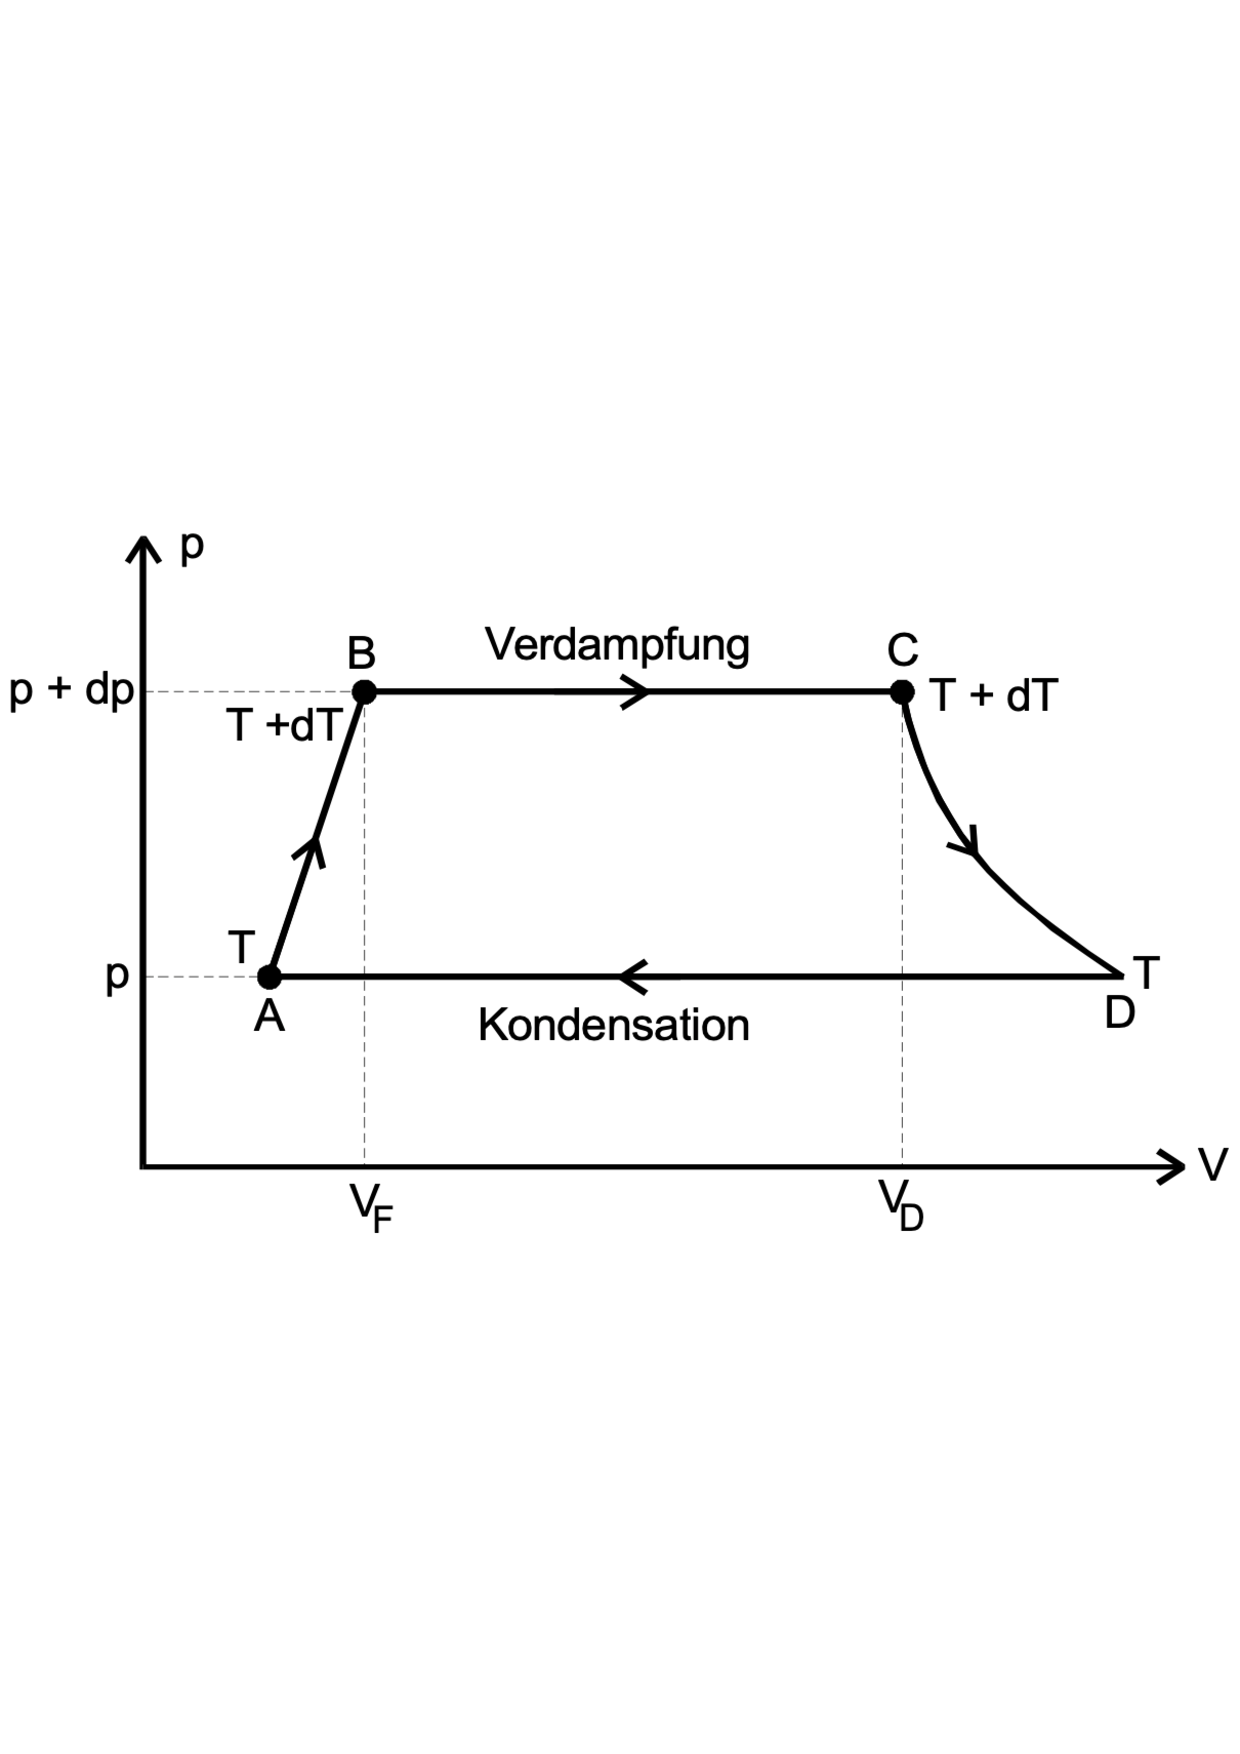
\includegraphics[width=8.5cm]{kreis.pdf}
    \caption{Kreisprozess der Verdampfung \cite{V203}.}
    \label{fig:kreis}
  \end{figure}

\noindent
Wird im Punkt A ein Mol Flüssigkeit um die Temperatur d$T$ erwärmt,
steigt der Druck um d$p$ und das Volumen auf $V_F$
und das System befindet sich nun in Punkt B.
Wenn die Wassermenge nach Zufuhr der Verdampfungswärme isotherm und isobar in Gas übergeht,
steigt das Volumen auf $V_D$ und das System befindet sich in Punkt C.
Durch Wärmeentzug wird der Dampf auf die Temperatur $T$ abgekühlt wobei der Druck wieder auf $p$ absinkt
und Zustand D ist erreicht.
Durch Zufuhr meschanische Energie wird der abgekühlte Dampf kondensiert und
Punkt A ist wieder erreicht.
Mit Überlegungen über die Molwärmen und Volumina im flüssigen und gasförmigen Zustand
kann mit dem zweiten Hauptsatz der Thermodynamik
und weiteren Umformungen die Clausius-Clapeyronsche Gleichung 

\begin{equation}
(V_D - V_F) \, \text{d}p = \frac{L}{T} \, \text{d}T
\label{eqn:clau}
\end{equation}

\noindent
hergeleitet werden.
Da $L$ in dem betrachteten Bereich der Dampfdruckkurve konstant ist, 
folgt durch Integration von Gleichung (\ref{eqn:clau}):

\begin{equation}
p = p_0 \, e^{-\frac{L}{RT}}
\label{eqn:claui}
\end{equation}